%*************************************************************************************************************************
\section{Uncertainty Quantification in Nuclear Engineering Thermal-Hydraulics}\label{sec:intro_uncertainty_quantification}
%*************************************************************************************************************************

% Introductory Paragraph
Before continuing the discussion of uncertainty analysis of code predictions, it will be worthwhile to define some additional terminologies to avoid later confusion.

In making a connection with the notion of \emph{simulator} introduced in Section~\ref{sec:intro_computer_simulation}, 
recall that from Fig.~\ref{fig:ch1_th_system_code} an \emph{input deck} is distinct from the code itself.
Fig.~\ref{fig:ch1_simulator_io} depicts the notion of simulator of a thermal-hydraulics system in a more generic way, as an input/output model.
\begin{figure}[bth]	
	\centering
	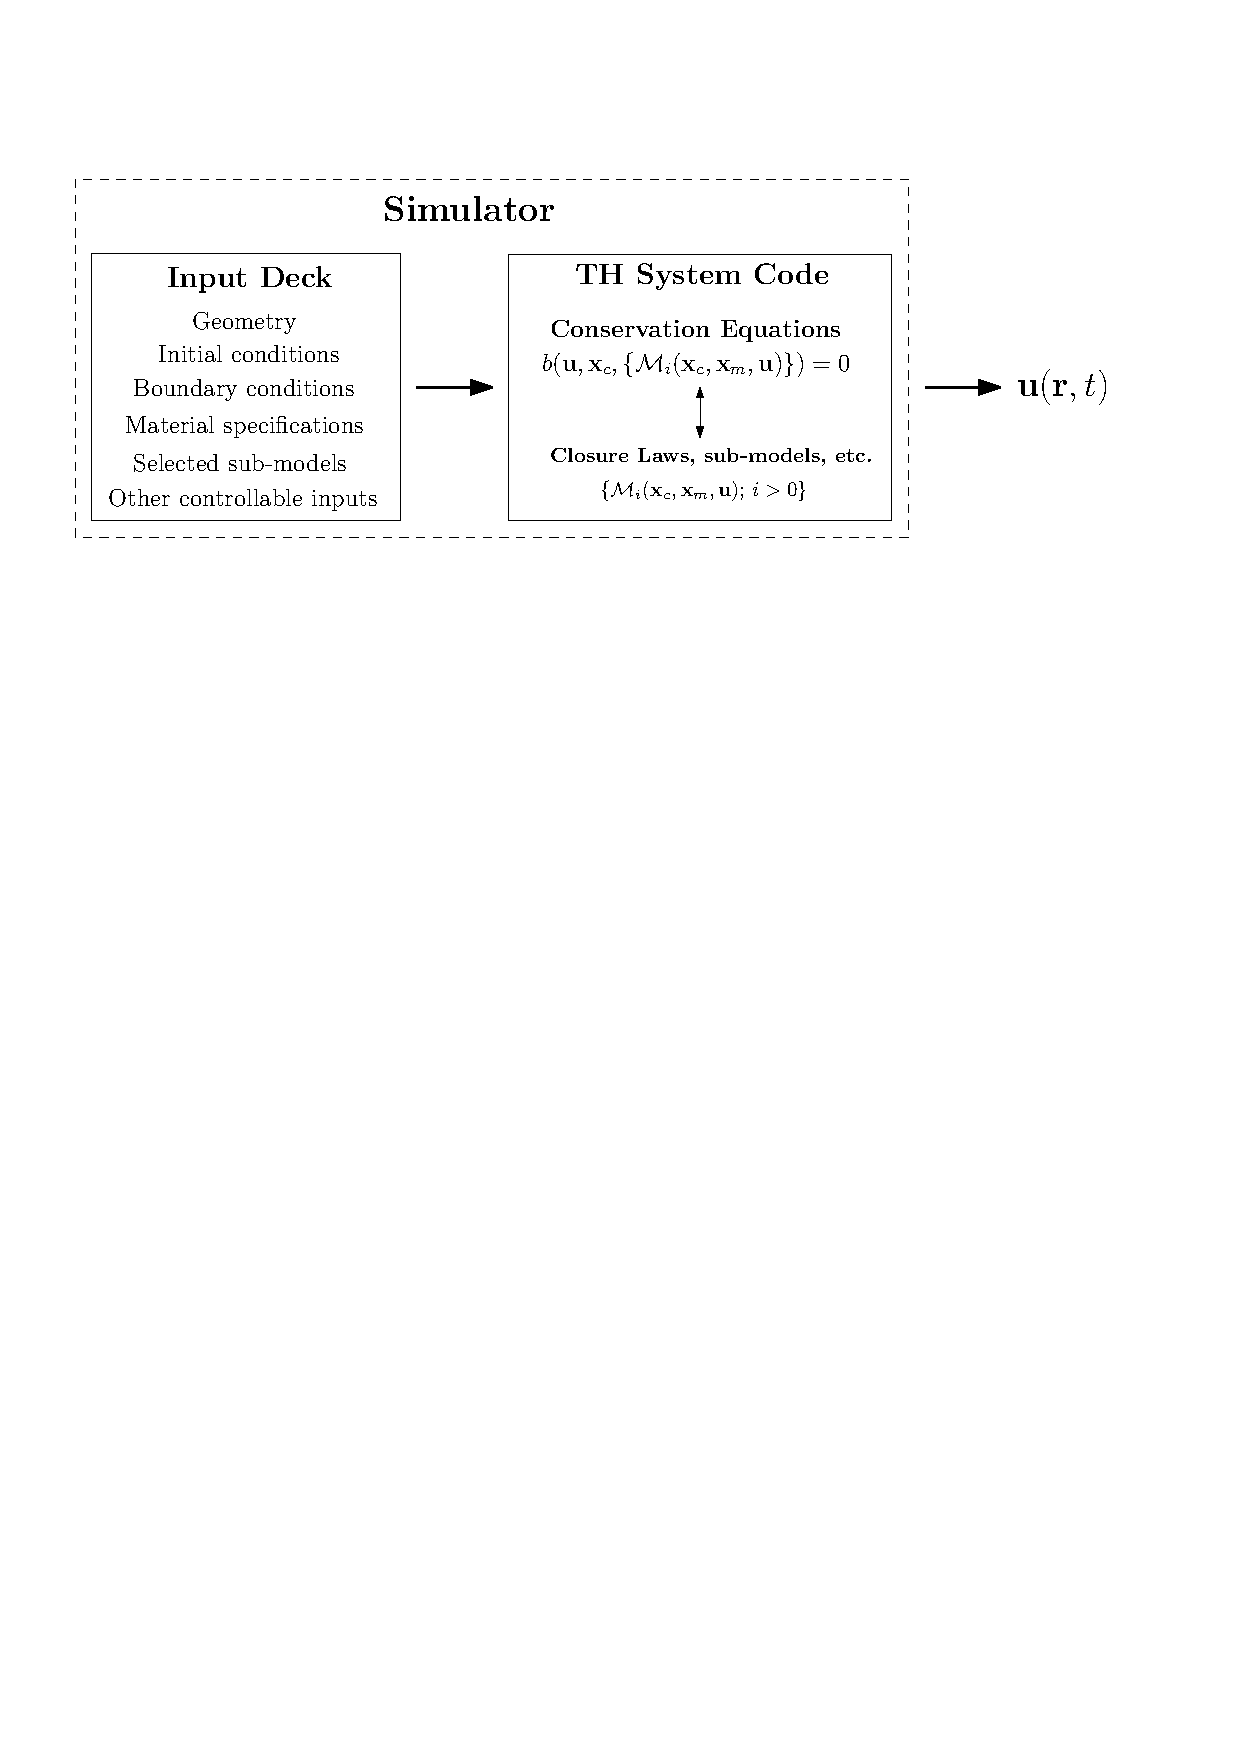
\includegraphics[width=\textwidth]{../figures/chapter1/figures/simulator_io}
	\caption[Simplified illustration of a simulator as an input/output model.]{Simplified illustration of a simulator as an input/output model.}
	\label{fig:ch1_simulator_io}
\end{figure}

Indeed input deck defines specific problem (i.e., system) of interest.
It includes the specifications for geometrical configuration (i.e., the nodalization), choice of material and fluid involves, as well as initial and boundary conditions.
It may also include the setting for the numerical solver.
\marginpar{Controllable inputs and model parameters}
Some of those specifications (such as the boundary conditions, etc.) are parametrized and constitutes \emph{controllable inputs} denoted by $\bm{x}_c$ that define a particular instance in which the simulator is to be used\footnote{later on, \emph{controllable} inputs correspond to the parameters whose counterparts in a physical experiment which can be controlled by the experimentalist.}.
The conservation equations of the code are closed with additional set of closure laws (and other sub-models) $\mathcal{M}_i(\bm{x}_c, \bm{x}_m, \bm{u})$.
These closure laws are, in turn, parametrized by a set of model specific parameters denoted by $\bm{x}_m$ which is referred to as the \emph{physical model parameters}.
Note that both the controllable inputs and the physical model parameters are considered by the code simply as \emph{inputs}.
 
Specifying the input deck, as far as user is concerned, completely defines the problem and the code will solve the conservation equations which output the dynamic state of relevant physical variables $\mathbf{u}(\bm{r}, t)$ (e.g., fluid pressure, temperature, wall temperature, etc.).
In practice, these raw simulation outputs are further post-processed to obtain the so-called \glspl[hyper=false]{qoi} the are relevant to the problem at hand.

%--------------------------------------------------------------------------
\subsection{Forward Uncertainty Quantification}\label{sub:intro_uq_forward}
%--------------------------------------------------------------------------

% Best-estimate, limitation
As explained, best-estimate analysis uses more realistic modeling assumptions for analyzing transient behavior of \gls[hyper=false]{npp}.
It attempts as realistically as possible to describe the behavior of the relevant physical processes occur during the plant transient.
And yet, even the best available understanding of the physical process is still limited.
Understanding of complex phenomena might not yet adequate and data support for some processes can be very limited.
Simplifying assumptions, approximations, and expert judgments to some degree are unavoidable and still required to have a complete analysis.

% Best-estimate, plus uncertainty
Hence, best-estimate analysis has to be complemented with uncertainty analysis.
\marginpar{Best-estimate plus uncertainty}
The ultimate goal of uncertainty analysis is to associate code prediction with its uncertainty.
These combined quantities are then compared with certain regulator safety limits (e.g., \gls[hyper=false]{pct}) to check whether the limits still fall outside the uncertainty band of the code prediction.

% Source of possible uncertainties
There are several known sources of uncertainty that render the prediction on $\bm{u}(\mathbf{r},t)$ and its derived quantities uncertain.
\marginpar{Sources of uncertainty}
The following are the sources of primary interest in the present research:
\begin{enumerate}

	\item \emph{Uncertainty associated with the controllable inputs}.
	In case of a controlled experiment, these controllable inputs are supposed to be observed (and \emph{controlled}).
	However, such an observation might contain observation error due to instrument imprecision and/or inherent variability. 
	In the case of simulation of a real accident scenario in a plant,
  some conditions of the plant parameters prior the accident scenario (the initial conditions) can also be measured.
  Furthermore, in such a scenario, controllable inputs may also include parameters that are part of the assumptions underpinning the deterministic safety analysis (i.e., conservative vs. best-estimate).
  This includes the boundary conditions, ranging from the availability of safety features to the constraints on their performance \cite{IAEA2002}.

  \item \emph{Uncertainty associated with the physical model parameters}.
	The value of the physical model parameters are often not known a priori.
	As such the uncertainty associated with them are epistemic in nature.
	They can either be estimated by using an experimental data from a calibration experiment or by expert judgment.
	
  \item \emph{Uncertainty associated with the physical models}.
	The physical models themselves are still approximations, even with perfectly known model parameters.
	If derived in fully mechanistic manner, it might be the case that some processes are unaccounted for due to inherent complexity and lack of knowledge (i.e., the case of \emph{missing physics}).
	On the contrary, if derived fully empirically, it might be the case that the models are derived separately for different more elementary processes, while in the applications of the code multiple of such models are used in concert. Despite each being validated, it is fair to question the validity of models used in an ensemble.
	Any of these tend to cause a systematic bias on the code prediction, the extend of which is unknown and uncertain.
	As a result, this source of uncertainty is referred to as model \emph{bias}, \emph{inadequacy}, or \emph{discrepancy}.

\end{enumerate}

% Forward uncertainty quantification, Inputs as random variables
In statistical uncertainty analysis, the controllable inputs and physical model parameters are modeled as random variables ($\bm{\mathcal{X}}_c$ and $\bm{\mathcal{X}}_m$, respectively) equipped with probability distributions.
\marginpar{Forward uncertainty quantification}
Then using \gls[hyper=false]{mc} technique, samples are generated from their respective distributions and they are used to run the code multiple times.
Finally, the resulting code outputs (raw or post-processed), are summarized to obtain the uncertainty measure of the prediction.
In other words, the uncertainties in the controllable inputs and physical model parameters are \emph{propagated forward} through the code to quantify the uncertainty of the predictions as shown in Fig.~\ref{fig:ch1_simulator_uq_forward}.
The practice of propagating parametric uncertainty by \gls[hyper=false]{mc} is widely accepted in the nuclear engineering thermal-hydraulics community \cite{Lellouche1990,Glaeser1994,Glaeser2008}.
\begin{figure}[!bth]	
	\centering
	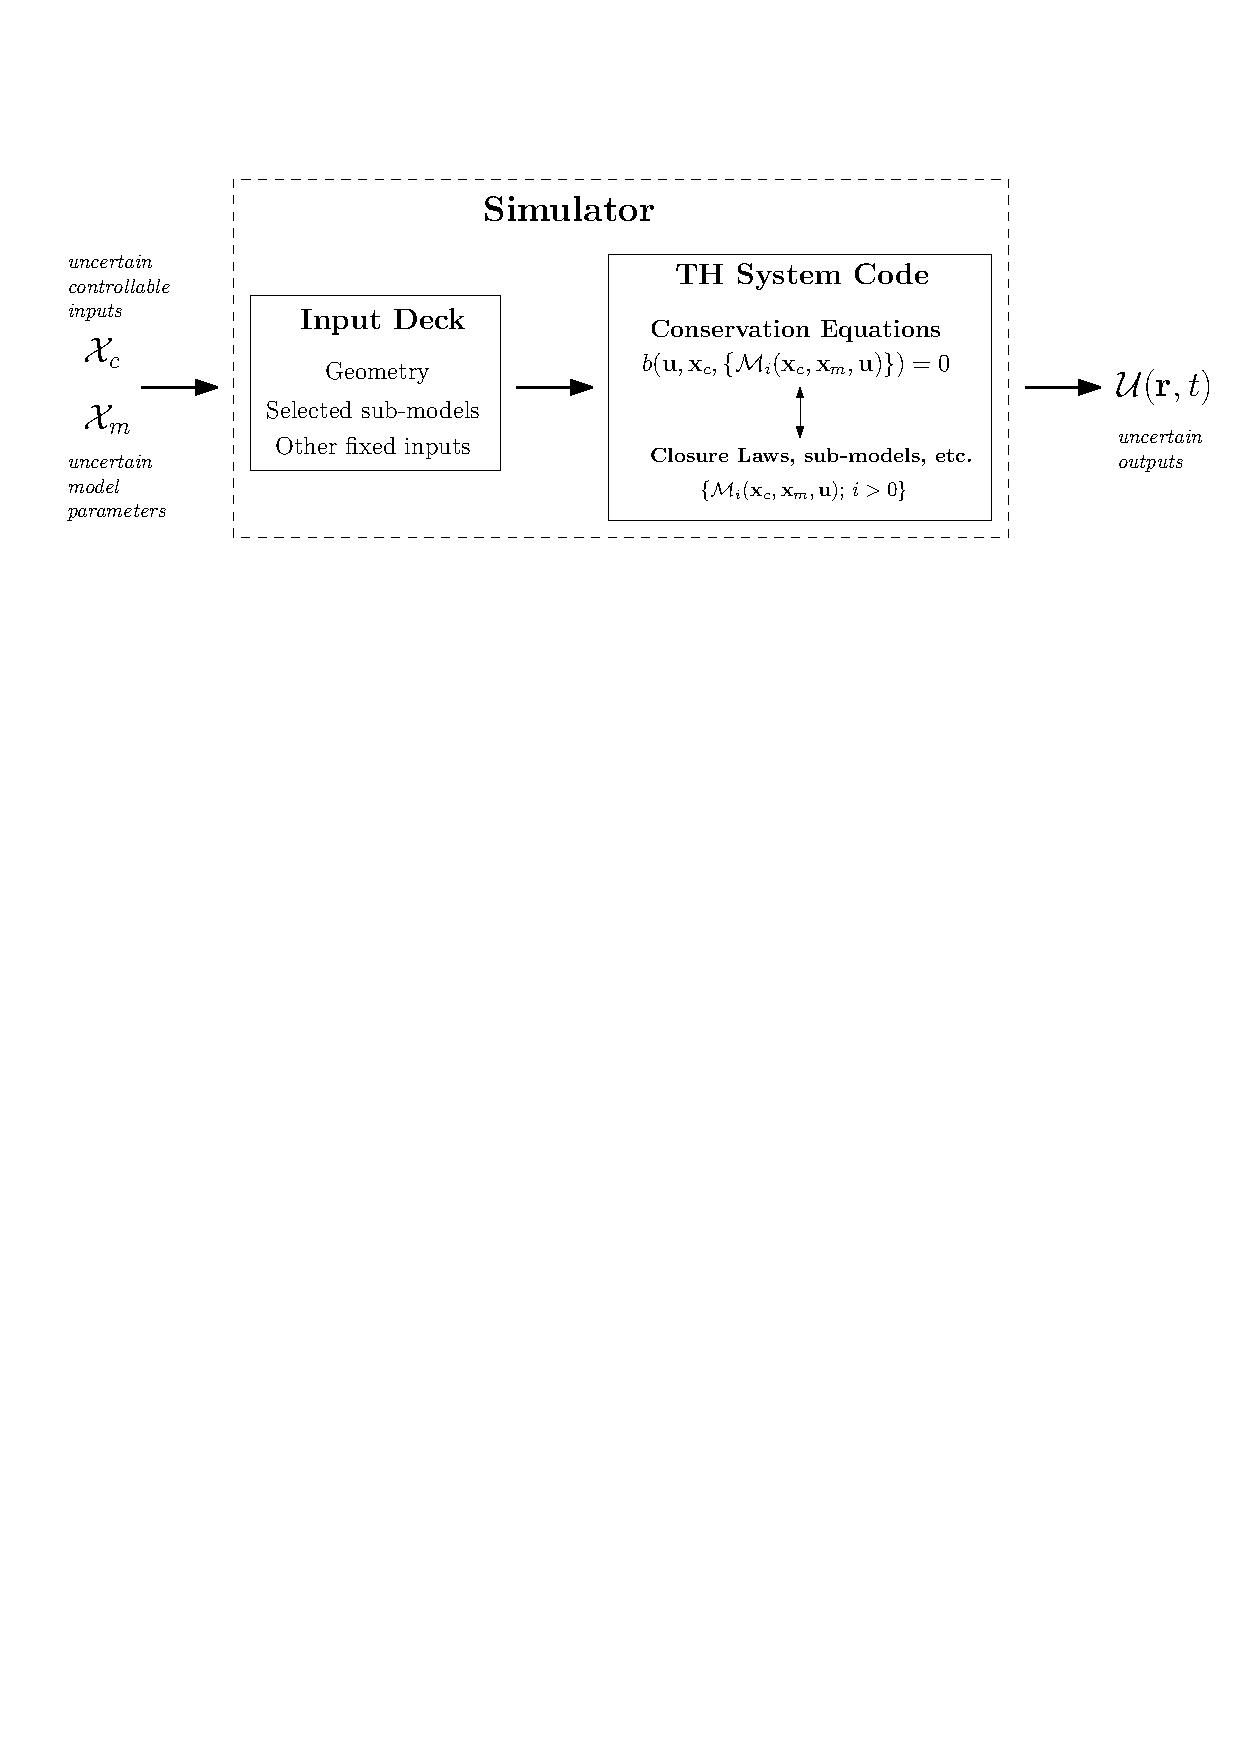
\includegraphics[width=\textwidth]{../figures/chapter1/figures/simulator_uq_forward}
	\caption[Simplified flowchart of forward uncertainty quantification of a simulator prediction.]{Simplified flowchart of forward uncertainty quantification of a simulator prediction. Notice that the simulator has been parametrized by the controllable inputs and physical model parameters, each of which are represented as random variable.}
	\label{fig:ch1_simulator_uq_forward}
\end{figure}

% Source of uncertainty, initial and boundary condition
The forward uncertainty quantification explained above deals with the parametric uncertainty associated with the important parameters of the simulator, both for the controllable inputs and the physical model parameters.
As a result, representing the  as random variables is the key in the forward uncertainty quantification of system code.

%--------------------------------------------------------------------------
\subsection{Inverse Uncertainty Quantification}\label{sub:intro_uq_inverse}
%--------------------------------------------------------------------------

% Model parameters
A lot has been said about the origin of the uncertainty associated with the controllable inputs.
The physical model parameters, however, are conceptually different.
\marginpar{Model parameters}
The physical models referred to in this thesis are usually represented either in the form of correlation, phenomenological (mechanistic) model, or a mixed between the two extremes (see Section~\ref{sub:intro_th_system_code}).
The parameters associated with the models can either represent physically meaningful quantities or not (This distinction will be revisited in Chapter~\ref{ch:bayesian_calibration}).
At this level, the uncertainty on these parameters depends on their origin or the approach used in the derivation.

% Representativity for NPP application
However it is worth considering that many of such models, be it empirical or mechanistic, were originally derived based on simplified systems (simplified geometry or limited flow conditions) \cite{Bestion2008}.
\marginpar{Separate Effect Test Facilities}
Consequently, to reflect more on the conditions of the reactor transient to be simulated,
experiment with well-specified conditions is conducted at \glspl[hyper=false]{setf}, facilities aimed at reproducing a particular safety-relevant phenomena during transient at a particular part of the reactor \cite{DAuria2012}.

The data is then used to assess the corresponding model (and possibly multiple models).
In the assessment against data from \glspl[hyper=false]{setf},
some parameters in the models are adjusted to match the experimental data \cite{Barre1990}.
\marginpar{Calibration against Separate Effect Test Facilities}
Alternatively, additional free parameters can also be introduced in the models to serve the same purpose \cite{Bestion2008}.
That is, the parameters are tuning parameters and become measures of the models inadequacy in reproducing the data.
Ultimately, some kind of optimal values for the parameters are estimated and implemented in the code.

% Origin of uncertainty
In light of this, it can be argued that the uncertainty associated with such parameters stems from the fact that the calibration was conducted only on selected data set obtained from a selected \gls[hyper=false]{setf}.
Different \glspl[hyper=false]{setf} for the same phenomena exist, covering wide range of flow configurations and experimental boundary conditions.
It is fair to ask whether the calibrated value will hold if the calibration were to be conducted in other \gls[hyper=false]{setf} for the same phenomena.

% Inverse uncertainty
To derive the uncertainty associated with the model parameters obtained in the manner above,
the problem can be posed as an inverse problem.
\marginpar{An inverse problem}
In this setting, given a set of experimental data $\{\mathbf{D}\}$ taken with known controllable inputs $\mathbf{x}_c$, the task is then to infer the value of the \emph{unobserved} parameters in the physical model used to predict the same quantity as the experimental data.
To avoid excessive bias to the calibration data, it is important here to acknowledge various sources of uncertainty previously mentioned:
experimental data and controllable inputs are observed but perhaps there remains residual variability and observation error associated with them;
and the associated models are also only approximations with a possible, but unknown, systematic bias.

% Bayesian framework
In a probabilistic setting, a natural way to make an inference of unobserved parameters based on observed data is
\marginpar{Inverse uncertainty quantification}
through the Bayes' theorem,
\begin{equation*}
	p(\bm{x}_m\,|\,\{\mathbf{D}\},\mathbf{x}_c) = \frac{p(\{\mathbf{D}\}\,|\,\bm{x}_m, \mathbf{x}_c) \cdot p(\bm{x}_m)}{\int p(\{\mathbf{D}\}\,|\,\bm{x}_m, \mathbf{x}_c) \cdot p(\bm{x}_m)\,d\bm{x}_m}
\end{equation*}
where the left-hand side of the equation signifies the posterior probability density conditioned on the observed data $\{\mathbf{D}\}$ and controllable inputs $\mathbf{x}_c$.
The right-hand side constitutes of the likelihood function $p(\{\mathbf{D}\}\,|\,\bm{x}_m, \mathbf{x}_c)$ (probability of observing data given the parameters), the prior of the model parameters $p(\bm{x}_m)$ (the initial state of knowledge regarding the parameters values before observing the data),
while the denominator signifies a normalizing constant such that the posterior is a valid \gls[hyper=false]{pdf} (that is, it integrates to one)\footnote{Note that the formulation assumes the controllable inputs $\mathbf{x}_c$ are fully known. If they are considered uncertain, such as in the case of variability, then a prior probability can be put on them as well.}.
Fig.~\ref{fig:ch1_simulator_uq_inverse} depicts a simplified flowchart of the inverse quantification described above.
\bigfigure[pos=tbhp,
           opt={width=1.0\textwidth},
           label={fig:ch1_simulator_uq_inverse},
           shortcaption={Simplified flowchart of inverse uncertainty quantification of model parameters.}]
{../figures/chapter1/figures/simulator_uq_inverse}
{Simplified flowchart of inverse quantification for model parameters of a simulator.}

The formulation and computation of the posterior above can be seen as a calibration exercise.
That is, it seeks to adjust the model parameters such that it is consistent with the observed data (i.e., calibration data) under the assumed likelihood and the prior.
\marginpar{Statistical calibration}
However, instead of obtaining a single estimated value (or values in case of multiple parameters), the resulting posterior is a \gls[hyper=false]{pdf}, conditioned on the observed data.
This posterior \gls[hyper=false]{pdf}, in turn, can be used in uncertainty propagation to quantify the uncertainty on the prediction made outside the calibration data set.
Note that, as tuning parameters, expert-judgment is often used to estimate the uncertainty on the parameters, measuring the degree of expected model performance through how much the model parameter is allowed to vary.
From this point of view, the approach uses the experimental data to better inform the prior expectation (or belief) about the model parameters values.

% Connection to PREMIUM Benchmark
The importance of characterizing the uncertainty in the physical models parameters was acknowledged by the \gls[hyper=false]{wgama} of the \gls[hyper=false]{oecd}/\gls[hyper=false]{nea}.
This led to the \gls[hyper=false]{premium} project.
Its main goal is to report the state-of-the-art of the available methodologies to quantify the uncertainty in the physical models parameters.
The following will briefly describe the project and highlight the main lessons learned from the author's perspective through his participation on behalf of the \glsfirst[hyper=false]{psi}.

%-------------------------------------------------------------
\subsection{OECD/NEA PREMIUM project}\label{sub:intro_premium}
%-------------------------------------------------------------

% Introductory paragraph
The \gls[hyper=false]{premium} project was an activity launched by the \gls[hyper=false]{oecd}/\gls[hyper=false]{nea} with the aim to advance the methods for quantifying the uncertainties associated with the physical model parameters in \gls[hyper=false]{th} system codes.
It was the continuation of the previous project \gls[hyper=false]{bemuse}, which concetrated on the propagation and sensitivity analysis of the input uncertainties in large scale simulation (\gls[hyper=false]{lbloca}).
The main finding of \gls[hyper=false]{bemuse} can be found in \cite{Perez2011}.
The emphasis of the \gls[hyper=false]{premium} benchmark was placed on the derivation of the model parameters uncertainty and their validation.

% Scope of the Project
The scope of the project was limited to the simulation of the phenomenon of core reflood and quenching under conditions representative of a \gls[hyper=false]{pwr} large break \gls[hyper=false]{loca}.
Experimental data from two \glspl[hyper=false]{setf} was made available for the purpose of uncertainty quantification of the model parameters as well as validation.
For the model parameters uncertainty quantification, the data from the \gls[hyper=false]{feba} reflood facility was used.
Although, the experimental data were taken at several controllable inputs (i.e., boundary conditions) in practice calibration was conducted using only one.
The derive uncertainties were then propagated and compared with the experimental data from other experimental runs of \gls[hyper=false]{feba} and from another reflood facility (PERICLES).
Thus the main goal of the project followed the approach of statistical uncertainty analyses explained above.

% Phase
Sixteen organizations from $11$ different countries participated in the $4$-year project ($2012$--$2016$) using $6$ different \gls[hyper=false]{th} system codes.
Each participant employing a chosen simulation code and methodology had to contribute to the $5$ following phases of the benchmark:
\begin{enumerate}
	\item \textsc{Phase 1}: Description of the selected simulation code and methodology.
  \item \textsc{Phase 2}: Identification of the uncertain parameters that are most relevant to \gls[hyper=false]{pwr} \gls[hyper=false]{loca} reflooding simulations.
  \item \textsc{Phase 3}: Quantification of the uncertainties if the parameters, using available data from the \gls[hyper=false]{feba} experiment.
  \item \textsc{Phase 4}: Propagation of the quantified uncertainties as part of a blind benchmark exercise based on data from the PERICLES experiment.
  \item \textsc{Phase 5}: Contribution to the analysis and synthesis of the benchmark results.
\end{enumerate}

% Lesssons learned
